\chapter{Inleiding}\label{ch:introductie}

Eiwitten of proteïnen zijn alomtegenwoordig en spelen een belangrijke rol in ons dagelijkse leven.
Ze garanderen een correcte werking van belangrijke processen binnen elk organisme.
Hieronder vallen de levensprocessen van ons eigen lichaam, maar ook die van dieren, planten, bacteriën en zelfs virussen.
Om deze processen te analyseren zijn er meerdere benaderingen mogelijk.


\section{Genomica, transcriptomica \& proteomica}\label{sec:genomica-transcriptomica-&-proteomica}
Een eerste mogelijkheid is aan de hand van het onderzoeksgebied van de \textbf{proteomica}.
Dit is de studie van alle eiwitten die binnen een enkel organisme tot expressie kunnen komen.
Hierbij probeert men te begrijpen hoe eiwitten in elkaar zitten, hoe deze met elkaar en binnen een bepaalde omgeving met elkaar interageren en wat hun belangrijkste functie is.
Naast proteomica bestaan er nog twee andere gerelateerde disciplines.
\\ \\
De eerste alternatieve discipline is \textbf{genomica}, het onderzoek naar het genoom.
Het genoom van een organisme is de collectie van al het DNA binnen een organisme.
Dit stelt voor welke proteïnen mogelijks door het organisme geconstrueerd kunnen worden.
Een belangrijk verschil met proteomica is dat DNA instructies voorstelt voor de productie van alle mogelijke proteïnen die het organisme kan maken.
Het geeft dus geen informatie over de proteïnen die op dat moment in de tijd actief zijn.
Het is een voorstelling van wat het organisme kan, niet wat het op \textit{dit} moment aan het doen is.
Belangrijk is dat ongeveer 98\% van het menselijke genoom niet-coderend is, wat wil zeggen dat dit deel van het DNA niet omgezet kan worden naar een betekenisvolle proteïne.
In de plaats kunnen ze wel omgezet worden naar \textit{regulatory sequences}, niet-coderende genen, of componenten die nog niet ontdekt zijn.
\\ \\
De andere discipline is de \textbf{transcriptomica}.
Deze discipline onderzoekt het transcriptoom van een organisme, wat de verzameling is van alle RNA moleculen die in het organisme aanwezig zijn.
Het transcriptoom is een belangrijke indicatie van welke delen uit het DNA effectief proteïnen encoderen.
Dit omdat RNA, meer specifiek messenger RNA (mRNA) en transfer RNA (tRNA), een belangrijk onderdeel is van het proces om DNA om te zetten naar proteïnen.
\\ \\
Onze focus ligt vooral binnen het veld van de \textbf{metaproteomica}.
Het \textit{meta} prefix zegt dat de te analyseren stalen niet van één organisme afkomstig zijn, maar van \textbf{meerdere organismen} (typisch binnen hetzelfde ecosysteem).
Dit maakt de analyse moeilijker aangezien proteïnen van verschillende organismen gelijkaardige aminozuursequenties kunnen hebben (al dan niet door toeval).
Meer specifiek is het doel van metaproteomica om op zoek te gaan naar de taxa en functies die horen bij een verzameling van peptiden.
Een een veelvoorkomende categorie van peptiden die we zullen analyseren zijn tryptische peptiden.


\section{Tryptische peptiden}\label{sec:tryptische-peptiden}
Tryptische peptiden zijn peptiden die ontstaan na het knippen van proteïnen aan de hand van \textbf{trypsine}.
Dit is een protease (eiwitafbrekend enzym) dat proteïnen opsplitst in meerdere peptiden.
Er bestaan nog andere proteases, maar trypsine is veruit de populairste door zijn eenduidig gedrag en efficiëntie.
\\ \\
Trypsine zal eiwitten knippen na elk voorkomen van lysine (K) of arginine (R) indien het eerstvolgende aminozuur geen proline (P) is.
Deze vuistregel is echter niet perfect.
Soms zal trypsine, een locatie waar normaal geknipt moet worden, missen.
Dit noemen we een \textit{missed cleavage}.
Figuur~\ref{fig:trypsine} bevat een voorbeeld van de werking.

\begin{figure}[H]
    \centering
    \includesvg[width=0.9\textwidth]{trypsine_verwerking}
    \caption{Voorbeeld van de werking van trypsine op 2 proteïnen~\cite{phdPieterUnipept}. De aminozuren in het rood zijn lysine (K) of arginine (R), waarna trypsine knipt (behalve als het eerstvolgende aminzoruur proline (P) is). De tweede proteïne bevat een voorbeeld waar niet geknipt wordt na lysine, doordat het opeenvolgende aminozuur proline is.}
    \label{fig:trypsine}
\end{figure}

Om de peptiden uit een experiment te kunnen gebruiken bij computeranalyses moeten deze omgezet worden naar een stringrepresentatie.
Dit is is echter een moeilijk en ingewikkeld proces.
Eerst wordt de massa/ladingsverhouding (m/z) van peptiden aan de hand van een massa spectrometer gemeten.
Daarna worden deze resultaten aan de hand van diverse zoekprocessen (via zogenaamde zoekmachines) omgezet naar de stringvoorstelling van de peptide.
Deze sequenties vormen de input voor tools zoals Unipept.


\section{Unipept}\label{sec:unipept-introductie}
Unipept~\cite{unipept_orig} biedt een ecosysteem van tools aan om stalen uit het onderzoeksveld van de metaproteomica te analyseren, maar er is ook een onderdeel (UMGAP~\cite{UMGAP_paper}) gericht op het analyseren van stalen uit de metagenomica.

\begin{itemize}
    \item \textbf{Unipept Web application~\cite{unipept_orig, unipept_web, unipept_tutorial, unipept_4}} Dit is de originele Unipept tool en is publiek beschikbaar op \url{https://unipept.ugent.be}.
    Met de gebruiksvriendelijke \textit{user interface} wordt analyseren van metaproteomica data beschikbaar gesteld.
    De resultaten van deze analyse worden aan de hand van visualisaties en tabellen aan de gebruiker voorgesteld.
    Deze kunnen vervolgens makkelijk geëxporteerd worden (bijv.~voor analyse in andere tools).
    \item \textbf{Unipept CLI~\cite{unipept_cli}} Dit is een \textit{power-user} tool om analyses uit te voeren op grotere stalen.
    \item \textbf{Unipept API~\cite{unipept_api, unipept_cli}} Dit is een collectie van \textit{endpoints} die andere applicaties, inclusief de CLI, toelaat om de functionaliteit van Unipept te integreren.
    \item \textbf{Unipept Desktop~\cite{unipept_desktop, unipept_desktop_2}} Dit is de recentste toevoeging aan het Unipept ecosysteem en laat toe dat onderzoekers niet noodzakelijk met de Unipept servers moeten communiceren om analyses uit te voeren.
    Deze applicatie combineert de voordelen van de web app, CLI en API en laat toe om lokaal stalen te analyseren, gebruikmakende van een gebruiksvriendelijke UI\@.

\end{itemize}

Op dit moment is Unipept \textbf{exclusief gericht op de analyse van tryptische peptiden}.
De reden hiervoor is de manier waarop de achterliggende indexstructuur opgebouwd wordt.
Dit opbouwen gaat in grote lijnen als volgt:

\begin{enumerate}
    \item Haal alle proteïnen en bijbehorende taxonomische en functionele annotaties op uit de UniProtKB databank~\cite{UniprotKB}.
    \item Splits deze proteïnen volgens de vuistregel die trypsine volgt.
    \item Sla alle resulterende tryptische peptiden op in een indexstructuur.
\end{enumerate}

Deze aanpak heeft als voordeel dat we op een efficiënte manier tryptische peptiden kunnen opzoeken (samen met de bijbehorende annotaties).
Er is echter een belangrijke keerzijde aan deze manier van werken.
Het zoeken van niet-tryptische peptiden (hieronder vallen ook peptiden met \textit{missed cleavage}) is problematisch.
Dit komt doordat tijdens het opbouwen van de Unipept indexstructuur de vuistregel gevolgd wordt, en elke peptide in de indexstructuur strikt tryptisch is.
Op basis hiervan worden de taxonomische annotaties voor elke tryptische peptide voorberekend.
\\ \\
Op dit moment is er wel een \textit{workaround} die toelaat om peptiden met \textit{missed cleavage} toch te zoeken.
Dit heeft echter wel een significante impact op de performantie.
Deze verminderde performantie bij \textit{missed cleavage}, in combinatie met het compleet ontbreken van een manier om willekeurig gesplitste peptiden te zoeken verklaart de nood aan een nieuwe indexstructuur.
\\ \\
Voor een gedetailleerdere beschrijving over Unipept en het onderzoeksveld van metaproteomica is het aangeraden om de inleiding van het doctoraat van Dr.~Pieter Verschaffelt te lezen~\cite{phdPieterUnipept}.
Dit vormde een duidelijke en goede basis voor deze inleiding.


\section{Probleemstelling}\label{sec:probleemstelling}
In deze masterproef zoeken we een oplossing voor het snel terugvinden van \textbf{willekeurige peptiden} in een eiwitdatabank.
Bij het vinden van een match moet het daarna mogelijk zijn de informatie op te halen die hoort bij alle proteïnen die matchen.
Binnen het onderzoeksgebied van de informatica kunnen we dit probleem als volgt herformuleren:
``In een grote verzameling van middellange strings (alle eiwitten in onze databank), moeten we voor een verzameling van korte strings (peptiden) terugvinden in welke van deze middellange strings ze voorkomen.''
We willen echter niet enkel vinden met welke proteïnes een peptide matcht.
Ook de bijbehorende taxonomische en functionele annotaties van de gematchte proteïnes moeten zo snel mogelijk te vinden zijn.
Hiervoor wordt waar mogelijk aggregaties van deze annotaties uitgevoerd tijdens het opbouwen van de indexstructuur.
\\ \\
Belangrijk hierbij is dat dit alles niet alleen \textbf{snel} gebeurt, maar we ook proberen \textbf{het vereiste geheugen tot een minimum te beperken}.
Wat als acceptabel beschouwd kan worden hangt af van de omgeving waarin de analyses uitgevoerd worden.
Voor stalen die geanalyseerd worden op een PC m.b.v~Unipept Desktop is dit $\pm$ 16 GB RAM\@.
Voor grotere stalen waarvan de analyse op de Unipept servers uitgevoerd wordt mikken we op 0.5-2 TB geheugenverbruik.
Dit komt overeen met een realistische configuratie voor een server die gericht is op het uitvoeren geheugenintensieve taken.
\\ \\
Tot slot willen we ook \textbf{inexacte matching} toevoegen tijdens het zoeken.
Door dit te doen kunnen we beter omgaan met kleine fouten die voorkomen tijdens het uitlezen van de experimentele stalen.
Om dit allemaal te bereiken is het doel van deze thesis om meerdere datastructuren uit te werken, te implementeren in Rust, en tot slot te testen.
Het gebruik van Rust laat ons toe om extreem hoge performantie te verkrijgen (vergelijkbaar met C en C++~\cite{rustPerformantie}) in combinatie met \textit{memory safety}\footnote{\textit{Memory safety} is een eigenschap die verzekert dat programma's enkel gebruik kunnen maken van geldige geheugenlocaties en geen \textit{undefined behaviour} zoals \textit{buffer overflows}, \textit{dangling pointers} en andere geheugen gerelateerde fouten kunnen vertonen.}.
Bovendien zijn sommige delen van Unipept al geschreven in Rust (zie UMGAP~\cite{UMGAP_paper, UMGAP_source}).
Dit laat toe om waar mogelijk bestaande code te hergebruiken.

\section{Benchmarkdatasets}\label{sec:datasets}
We gebruiken 2 soorten benchmarkbestanden.
De eerste soort zijn de proteïnedatabanken waarmee we de indexstuctuur opbouwen.
De grootte van deze indexstructuur is het primaire criterium aangezien deze in volledig in het RAM-geheugen moet passen, wat een harde limiet is.
Indien de index niet in het geheugen raakt zal het programma niet uitgevoerd kunnen worden (of met een erg grote performance-penalty wanneer \texttt{swap}\footnote{Dit is wanneer een computer schijfruimte gebruikt om het tekort aan RAM geheugen op te vangen.} gebruikt wordt).
De andere soort bestanden bevatten de peptides die we gaan proberen terugvinden in de indexstructuur.
Deze worden gebruikt om de zoekperformantie te testen.
Dit is een zachte limiet aangezien we mikken voor hoge performantie, maar tragere code heeft enkel als gevolg dat een gebruiker langer moet wachten.
Alle bestanden die in de volgende secties besproken worden kunnen teruggevonden worden onze GitHub repository\footnote{\url{https://github.com/BramDevlaminck/Thesis_benchmarkdata}}.

\subsection{Proteïnedatabanken}\label{subsec:proteine-databanken}
Om te testen hoe goed een implementatie is en hoe deze zich verhoudt ten opzichte van bestaande implementaties is het belangrijk om representatieve datasets te gebruiken.
Deze datasets zijn allemaal eiwitdatabanken die een subset vormen van UniProtKB (meer specifiek UniProtKB 2023\_04)~\cite{UniprotKB}.
UniProt zelf bestaat uit twee onderdelen (gegeven statistieken zijn voor release 2023\_04).
\begin{enumerate}
    \item Swiss-Prot: Dit is een kleinere, manueel gecureerde dataset met 570 157 eiwitsequenties.
    \item TrEMBL: Deze dataset bevat 251 600 768 sequenties en is dus veel groter dan Swiss-Prot.
    Een bijkomend verschil is dat deze dataset \textbf{niet} manueel gecureerd is, maar algoritmisch geannoteerd werd.
\end{enumerate}
Het einddoel van deze masterproef is om een index op te bouwen voor UniProtKB\@.
Daarmee bedoelen we de unie van Swiss-Prot en TrEMBL\@.
Dit is echter veel te groot om mee te werken tijdens het testen.
In de plaats gebruiken we tijdens het ontwikkelen twee kleinere subsets van UniProtKB\@.
Eerst wordt een overzicht gegeven van de belangrijkste eigenschappen van UniProtKB, om daarna dieper in te gaan op de twee gebruikte subsets tijdens het testen.

\paragraph{UniProtKB}
Tabel~\ref{tab:uniprotKB_eigenschappen} bevat een overzicht van de belangrijkste statistieken voor de volledige UniProtKB 2023\_04 databank.
Belangrijk om op te merken is dat de totale databank uit 86 805 673 041 aminozuren bestaat.
Omgerekend is dit 86,81 GB aangezien 1 karakter opgeslagen wordt in 1 byte.
Dit ondersteunt onmiddellijk de keuze om gebruik te maken van kleinere datasets tijdens het testen.

\begin{table}[h!]
    \centering
    \begin{tabular}{ l l }
        Metriek                   & Waarde            \\
        \hline\hline
        Totaal aantal sequenties  & 248 842 516       \\
        Totale lengte             & 86 805 673 041 aa \\
        Minimale proteïnelengte   & 1 aa              \\
        Maximale proteïnelengte   & 45 354 aa         \\
        Gemiddelde proteïnelengte & 348.84 aa         \\
        Mediaan proteïnelengte    & 278 aa            \\
        \hline
    \end{tabular}
    \caption{Eigenschappen van de volledige UniProtKB 2023\_04 databank. De afkorting \textit{aa} staat voor \textit{amino acids}.}
    \label{tab:uniprotKB_eigenschappen}
\end{table}

\paragraph{Swiss-Prot} Deze databank is één van de twee standaard onderdelen van UniProt.
Een kort overzicht van alle statistieken is terug te vinden in Tabel~\ref{tab:swissprot_eigenschappen}.
Figuur~\ref{fig:swissprot_aminozuur} en Figuur~\ref{fig:swissprot_length} geven meer inzicht in de distributie van de aminozuren en lengte van de proteïnen.

\begin{table}[h]
    \centering
    \begin{tabular}{l l}
        Metriek                   & Waarde         \\
        \hline\hline
        Totaal aantal sequenties  & 569 619        \\
        Totale lengte             & 205 954 074 aa \\
        Minimale proteïnelengte   & 2 aa           \\
        Maximale proteïnelengte   & 35 213 aa      \\
        Gemiddelde proteïnelengte & 361.56 aa      \\
        Mediaan proteïnelengte    & 295 aa         \\
        \hline
    \end{tabular}
    \caption{Eigenschappen van de Swiss-Prot databank (UniProt 2023\_04).}
    \label{tab:swissprot_eigenschappen}
\end{table}


\begin{figure}[h]
    \centering
    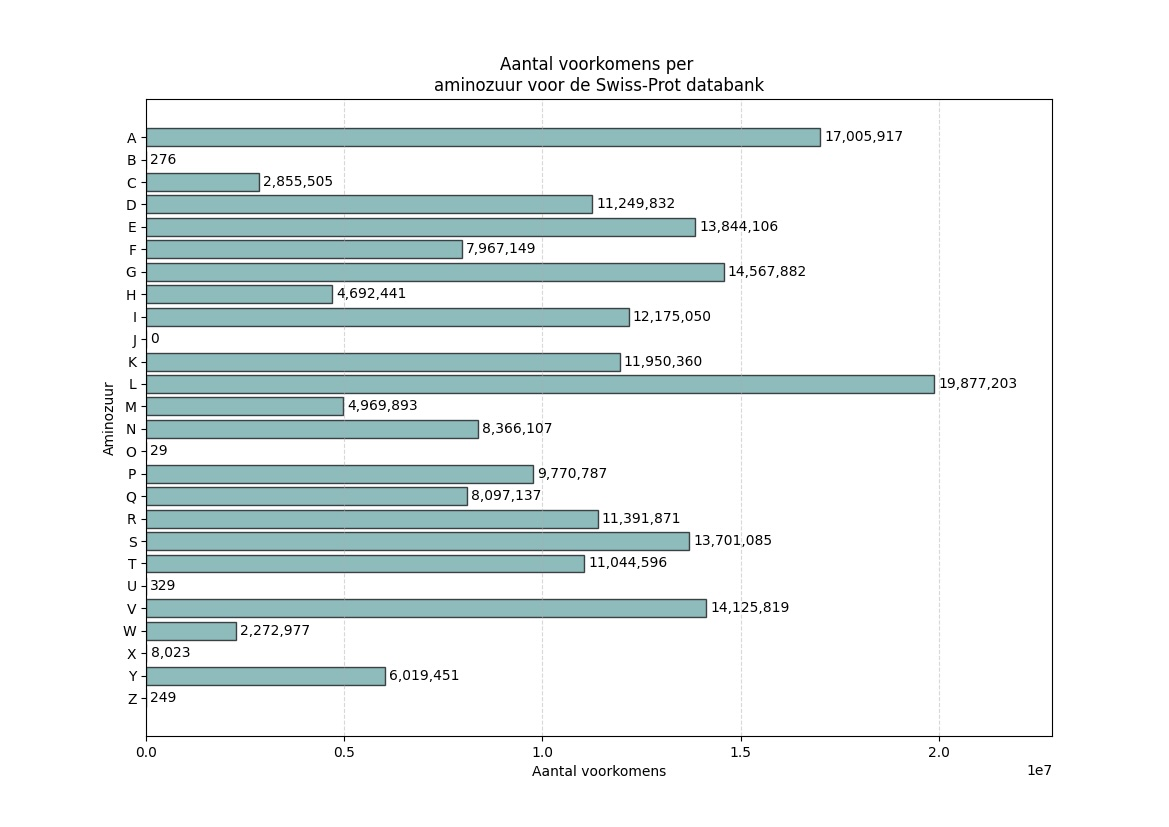
\includegraphics[width=0.6\linewidth]{swissprot_aminozuur_voorkomens}
    \caption{Aantal voorkomens per aminozuur voor alle proteïnen in de Swiss-Prot databank uit UniProt 2023\_04.}
    \label{fig:swissprot_aminozuur}
\end{figure}

\begin{figure}[h]
    \centering
    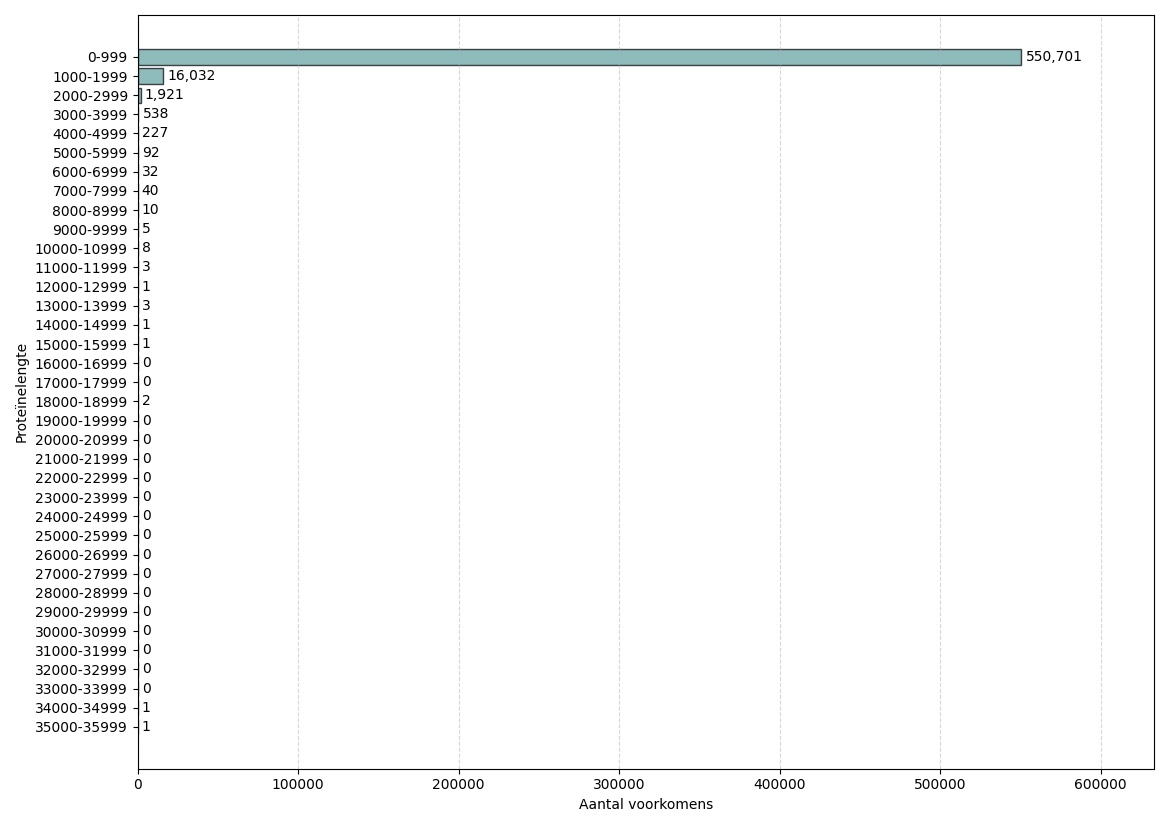
\includegraphics[width=0.95\linewidth]{swissprot_length_distribution_large}
    \makebox[0pt][r]{% Similar to \llap
        \raisebox{2.2em}{%
            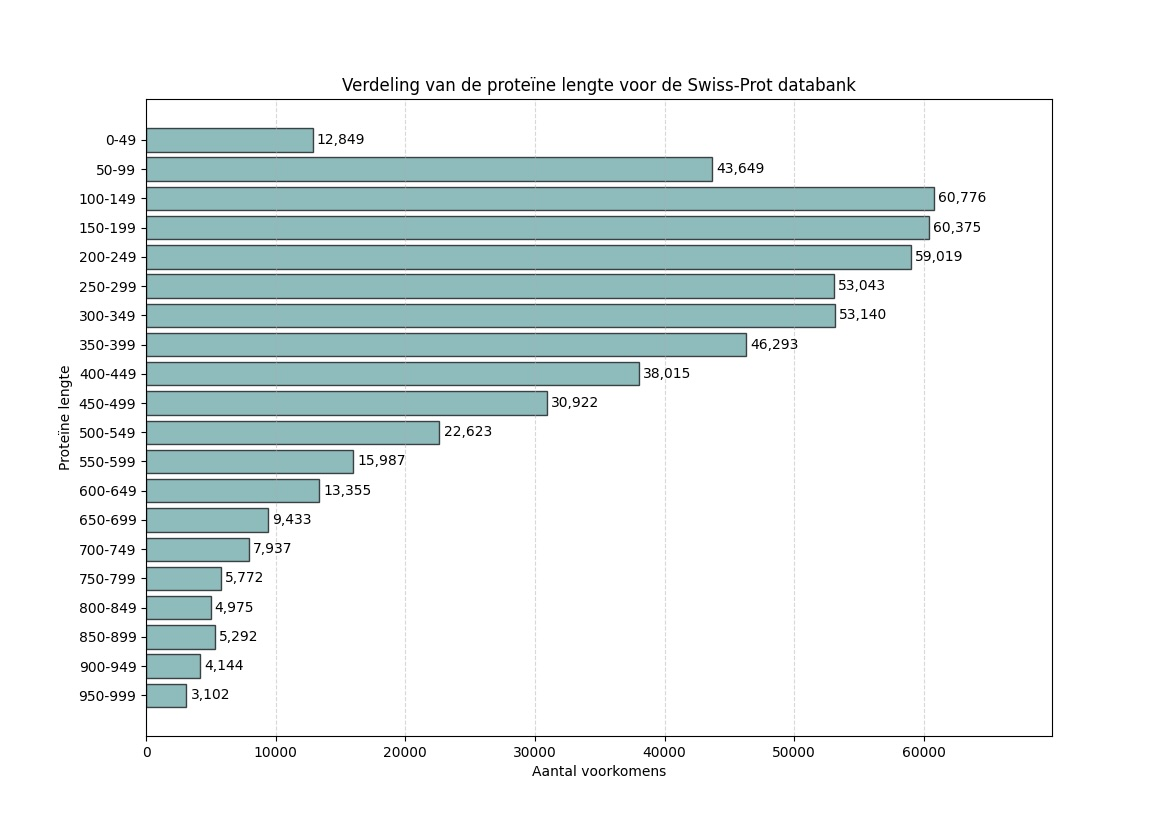
\includegraphics[width=0.65\linewidth]{swissprot_length_distribution_small}% Inserted image/inset
        }\hspace*{2em}%
    }%
    \caption{Lengtedistributie van de proteïnen in de Swiss-Prot databank. De kleinere grafiek bevat een gedetailleerder overzicht van de distributie in het interval $[0, 1000[$.}\label{fig:swissprot_length}
\end{figure}

Doordat het gebruikte invoerbestand reeds verwerkt werd door een deel van de Unipept pipeline, is er een klein verschil tussen het totaal aantal sequenties in Tabel~\ref{tab:swissprot_eigenschappen} en wat eerder aangegeven werd.
Hierbij worden onder andere sequenties met een onbekend taxon id verwijderd, wat het kleine verschil verklaart.

\paragraph{Human-Prot} Deze dataset is samengesteld aan de hand van drie referentiedatabanken afkomstig uit UniProtKB\@.
Dit zijn de Human Genome~\cite{proteomes_homo_sapiens}, Influenza B~\cite{proteomes_infuenza_b} en Human Papillomavirus~\cite{proteomes_human_papillomavirus} databank.
Opnieuw komen deze allemaal uit UniProt 2023\_04.
\\ \\
Deze Human-Prot databank is kleiner dan Swiss-Prot, waardoor het testen tijdens ontwikkeling sneller is.
Tabel~\ref{tab:humanprot_eigenschappen} somt enkele belangrijke metrieken op over deze dataset.
Figuur~\ref{fig:humanprot_aminozuur} en~\ref{fig:humanprot_length} gaan dieper in op een aantal details.

\begin{table}[h!]
    \centering
    \begin{tabular}{ l l }
        Metriek                   & Waarde        \\
        \hline\hline
        Totaal aantal sequenties  & 82 695        \\
        Totale lengte             & 30 293 046 aa \\
        Minimale proteïnelengte   & 2 aa          \\
        Maximale proteïnelengte   & 35 991 aa     \\
        Gemiddelde proteïnelengte & 366.32 aa     \\
        Mediaan proteïnelengte    & 204 aa        \\
        \hline
    \end{tabular}
    \caption{Eigenschappen van de Human-Prot databank (UniProt 2023\_04).}
    \label{tab:humanprot_eigenschappen}
\end{table}

\begin{figure}[H]
    \centering
    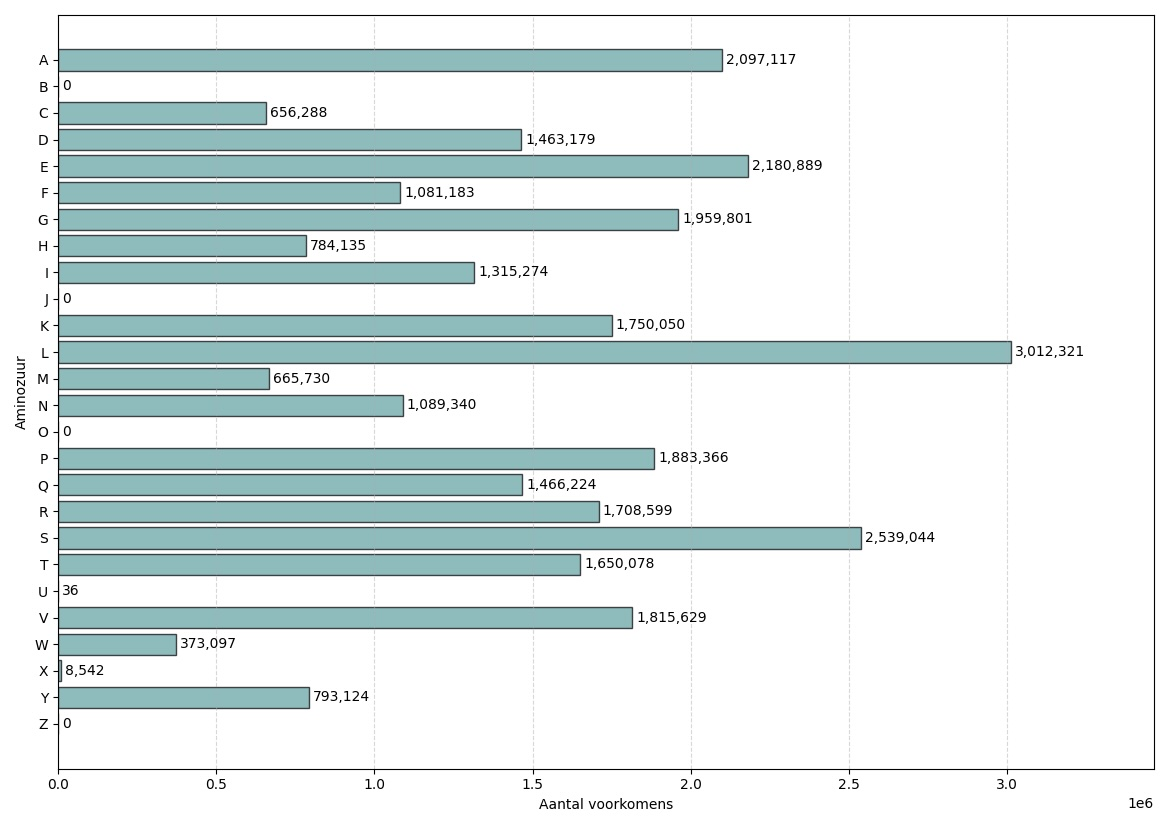
\includegraphics[width=0.7\linewidth]{humanprot_aminozuur_voorkomens}
    \caption{Aantal voorkomens per aminozuur voor alle proteïnen in de Human-Prot databank.}
    \label{fig:humanprot_aminozuur}
\end{figure}

\begin{figure}[h]
    \centering
    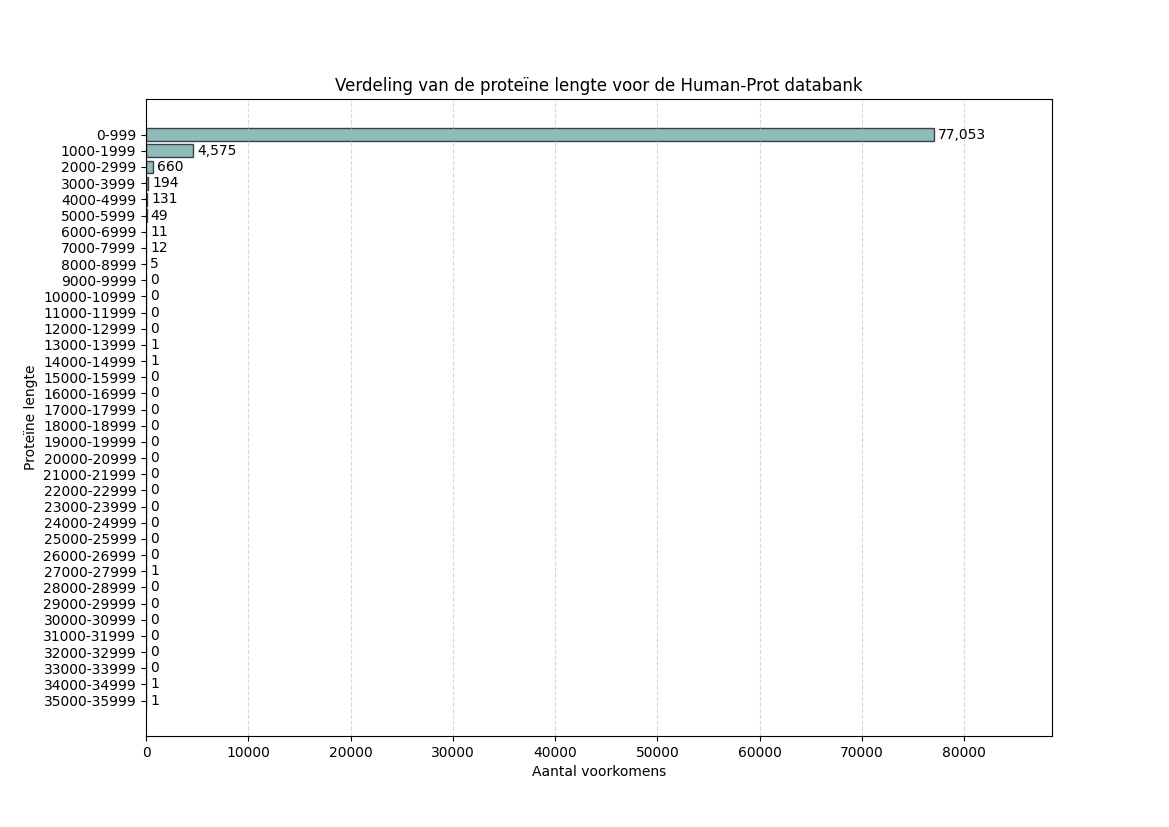
\includegraphics[width=0.95\linewidth]{humanprot_length_distribution_large}
    \makebox[0pt][r]{% Similar to \llap
        \raisebox{2.2em}{%
            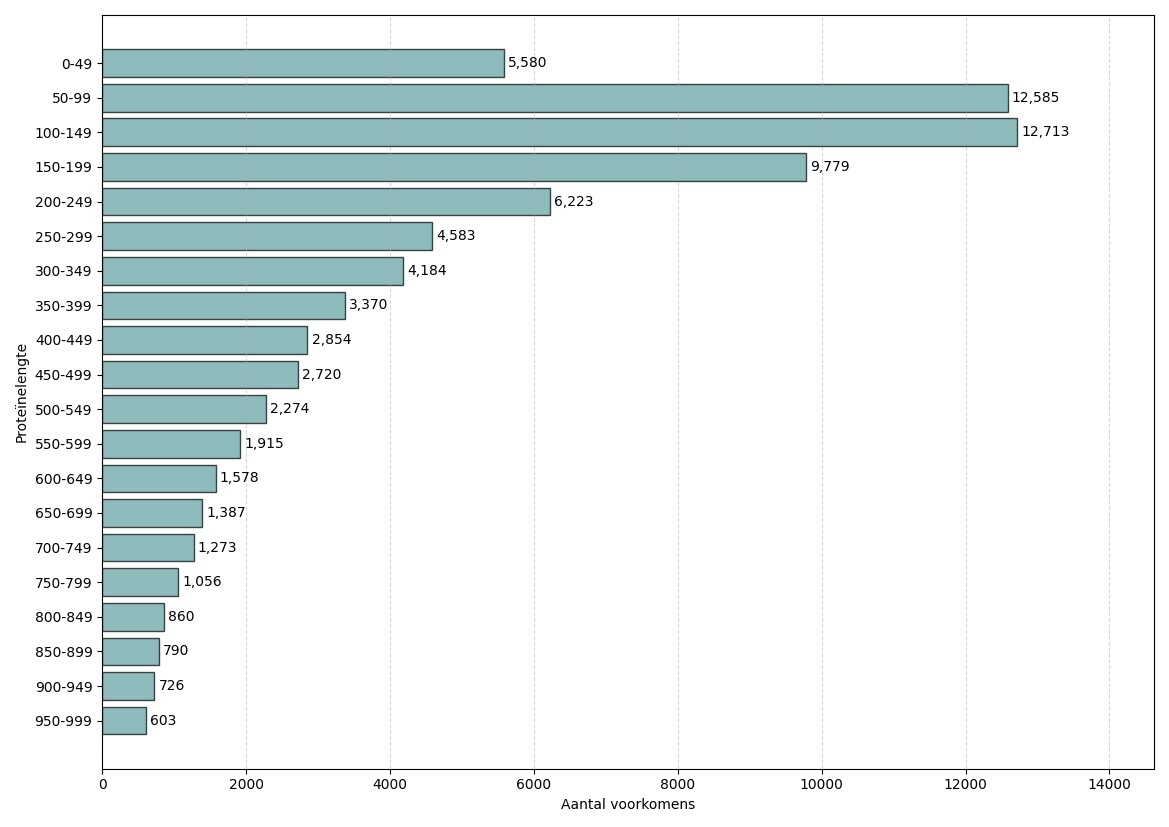
\includegraphics[width=0.65\linewidth]{humanprot_length_distribution_small}% Inserted image/inset
        }\hspace*{2em}%
    }%
    \caption{Lengtedistributie van de proteïnen in de Human-Prot databank. De kleinere grafiek bevat een gedetailleerder overzicht van de distributie in het interval $[0, 1000[$.}\label{fig:humanprot_length}
\end{figure}

We kunnen concluderen dat zo goed als alle letters gebruikt worden (ook al zijn er maar 20 aminozuren).
Dit komt doordat sommige letters eigenlijk een soort wildcard voorstellen.
Zo staat ``X'' voor elk mogelijk aminozuur, ``Z'' voor ``Q'' of ``E'',\ldots
\\ \\
Verder valt ook te zien dat de verdeling van de proteïnelengtes in de UniProtKB, Swiss-Prot en Human-Prot datasets vergelijkbaar zijn.
Dit laat ons toe om gebruik te maken van de Swiss-Prot en Human-Prot eiwitdatabanken en later de resultaten te veralgemenen naar UniProtKB\@.

\subsection{Peptidebestanden}\label{subsec:peptide-zoek-bestanden}
De zoekperformantie van onze indexstructuur is een erg belangrijk aspect.
Om dit te meten hebben we bij elke eiwitdatabank een lijst aan peptiden die we proberen te zoeken.
Voor beide databanken zijn enkele datasets opgesteld.

\subsubsection{Swiss-Prot}
Voor deze proteïnedatabank hebben we enkele peptidebestanden voorzien.
Twee bestanden die gesampled zijn en een reeks aan real-life stalen.
De twee artificiële bestanden zijn zo gekozen dat de ene enkel tryptische peptiden bevat, terwijl de andere ook peptiden bevat met \textit{missed cleavages}.
De eerste kan dus op dit moment al efficiënt door Unipept verwerkt worden, terwijl dit voor de tweede niet mogelijk is.

\paragraph{Artificiële stalen}
Tabel~\ref{tab:artifiele_bestanden_statistieken} bevat in kolom twee en drie een kort overzicht met statistieken voor deze gesamplede bestanden.

\begin{table}[H]
    \centering
    \begin{tabular}{l l l l}
        Metriek                    & Swiss-Prot-NOMC & Swiss-Prot-MC & Human-Prot       \\
        \hline\hline
        Totaal aantal sequenties   & 100 000         & 100 000       & 250 000          \\
        Totale lengte              & 1 605 909 aa    & 2 544 356 aa  & 2 458 834 046 aa \\
        Minimale peptidelengte     & 5 aa            & 5 aa          & 1 aa             \\
        Maximale peptidelengte     & 50 aa           & 93 aa         & 12 aa            \\
        Gemiddelde peptidelengte   & 16.06 aa        & 25.44 aa      & 9.84 aa          \\
        Mediaan peptidelengte      & 13 aa           & 23 aa         & 10 aa            \\
        Aantal vindbare peptiden   & 67 375          & 62 581        & 250 000          \\
        Aantal tryptische peptiden & 100 000         & 4107          & 102 659          \\
        \hline
    \end{tabular}
    \caption{Eigenschappen van de verschillende peptidebestanden. \textit{Swiss-Prot-NOMC} bevat de statistieken voor het Swiss-Prot peptidebestanden zonder \textit{missed cleavages}, terwijl \textit{Swiss-Prot-MC} net wel \textit{missed cleavages} bevat. De laatste kolom bevat de statistieken voor het peptidebestand dat hoort bij de Human-Prot eiwitdatabank.}
    \label{tab:artifiele_bestanden_statistieken}
\end{table}

\paragraph{Experimentele stalen}
Om de performantie beter te beoordelen, gebruiken we ook enkele stalen uit experimenten met een kleine micro-organisme gemeenschap, namelijk SIHUMIx\footnote{Simplified human intestinal microbiota}~\cite{SIHUMI_first_introduction, SIHUMI_frequently_used}.
Aangezien dit effectieve stalen zijn, bevatten deze \textit{missed cleavages} die natuurlijk ontstaan zijn.
Tabel~\ref{tab:sihumi_zoekbestanden} bevat de belangrijkste statistieken voor elk peptidebestand.
Deze peptidebestanden worden in combinatie met de Swiss-Prot proteïnedatabank gebruikt tijdens het testen.

\begin{table}[ht]
    \begin{minipage}{\linewidth}
        \centering
        \resizebox{\textwidth}{!}{ % use resizebox to textwidth since this needs to be scaled down in size a bit because otherwise it does not fit on the width of the screen
        \begin{tabular}{ l l l l l l l }
            Metriek                    & SIHUMI 03  & SIHUMI 05  & SIHUMI 05  & SIHUMI 08  & SIHUMI 11  & SIHUMI 14  \\
            \hline\hline
            Totaal aantal sequenties   & 25 000     & 25 000     & 24 424     & 25 000     & 24 998     & 25 000     \\
            Totale lengte              & 420 544 aa & 420 423 aa & 373 633 aa & 316 114 aa & 366 894 aa & 430 674 aa \\
            Minimale peptidelengte     & 6 aa       & 6 aa       & 6 aa       & 6 aa       & 6 aa       & 6 aa       \\
            Maximale peptidelengte     & 50 aa      & 50 aa      & 47 aa      & 43 aa      & 50 aa      & 50 aa      \\
            Gemiddelde peptidelengte   & 16.82 aa   & 16.82 aa   & 15.30 aa   & 12.64 aa   & 14.68 aa   & 17.23 aa   \\
            Mediaan peptidelengte      & 15 aa      & 16 aa      & 14 aa      & 12 aa      & 14 aa      & 16 aa      \\
            Aantal vindbare peptiden   & 2570       & 2698       & 3652       & 4135       & 3792       & 2761       \\
            Aantal tryptische peptiden & 17 263     & 162        & 152        & 207        & 153        & 242        \\
            \hline
        \end{tabular}}
    \caption{Eigenschappen van de SIHUMIx peptidebestanden. Elke kolom stelt een staal voor met als bestandsnaam \texttt{S<XX>.txt}. Deze stalen kunnen teruggevonden worden in onze GitHub repository \protect\footnote{\url{https://github.com/BramDevlaminck/Thesis\_benchmarkdata}} onder de \texttt{SIHUMI}-folder.} % protect is needed to make footnote possible in a caption. This is combined with a minipage to place the footnote directly under the table
    \label{tab:sihumi_zoekbestanden}
    \end{minipage}
\end{table}


\subsubsection{Human-Prot}
Voor deze databank hebben we één peptidebestand bestaande uit HLA-peptiden.
Dit zijn korte, niet-tryptische peptiden uit het immunopeptidomics onderzoeksveld.
Hierdoor kan Unipept op dit moment niet gebruikt worden om dit soort stalen te analyseren.
Elke peptide in dit peptidebestand is een sample van een proteïne uit de Human-Prot databank.
Hierdoor zijn alle peptiden die we zoeken effectief vindbaar in de dataset.
Een kort overzicht van enkele eigenschappen is terug te vinden in de laatste kolom van tabel~\ref{tab:artifiele_bestanden_statistieken}.
\\ \\
Appendix~\ref{ch:appendix-statistieken-zoekbestanden} bevat aanvullende grafieken over bovenstaande peptidebestanden.
Deze tonen voor elk peptidebestand de distributie van de aminozuren en de distributie van de peptidelengte.


\section{Benchmark hardware}\label{sec:benchmark-hardware}
Alle benchmarks werden uitgevoerd op een virtuele machine van team Unipept.
Tabel~\ref{tab:Matt_hardware} bevat een overzicht van de hardware van de fysieke machine en hoeveel toegekend is aan de VM\@.
Al deze informatie, en ook over de andere machines gebruik door Unipept, kan teruggevonden worden op de Unipept GitHub wiki~\cite{unipept_infrastructure}.

\begin{table}[h!]
    \centering
    \begin{tabular}{p{0.20\linewidth}p{0.45\linewidth}p{0.25\linewidth}}
        Onderdeel         & Fysieke server                                                            & Virtuele Machine    \\
        \hline\hline
        CPU               & 2x Intel Xeon 4410Y (12 cores / 24 threads, 2 - 3.9 GhZ, 30 MiB cache)    & 12 threads          \\
        RAM               & 768 GiB                                                                   & 128 GiB             \\
        Opslag            & 6x 16 TiB HDD (3.5 inch, 7.2K RPM SATA), 4x 3.84 TiB SSD (2.5 inch, SATA) & 1 TiB SSD, 4TiB SSD \\
        Besturingssysteem & Debian 12 (met Proxmox)                                                   & Ubuntu 22.04 LTS    \\
        \hline
    \end{tabular}
    \caption{Hardwarespecificaties van de fysieke server en virtuele machine die gebruikt worden tijdens het testen. Deze virtuele machine draait samen met nog enkele andere VMs op de server.}
    \label{tab:Matt_hardware}
\end{table}

Naast deze VM hebben we ook toegang tot enkele andere machines indien hier nood toe zou zijn.
Het is mogelijk in het totaal 768 GiB aan RAM kunnen ter beschikking stellen op een Unipept machine door enkele VMs en Unipept applicaties te verdelen over andere machines.
De HPC van UGent\footnote{https://docs.hpc.ugent.be/Linux/} biedt nodes aan die tot 940 GiB aan RAM hebben.
Tot slot heeft de CompOmics\footnote{Computational Omics} onderzoeksgroep aan UGent ook enkele machines staan dit tot 2TiB aan geheugen hebben.
Deze onderzoeksgroep werkt aan softwaretoepassingen voor het verwerken van proteomica-data, waar het onderzoeksgebied van de metaproteomica onder valt.
